\section*{Introduction}
Soit une poutre de section carré et de longueur "infinie" soumise à une charge $F$. On se propose d'étudier la résistance de cette poutre lorsqu'elle est chargée verticalement. On définie le champs de contraintes $\sigma = \begin{pmatrix}
\sigma_{xx} & \sigma_{xy}\\
\sigma_{xy} & \sigma_{yy}
\end{pmatrix}$. On souhaite maximiser la charge imposée (c'est à dire l'intégrale de $\sigma_{yy}$ sur la surface supérieur de la poutre) sans qu'il y ait déformation plastique, sous les contraintes mécaniques suivantes : 
\begin{align}
\frac{\partial \sigma_{xx}}{\partial x} + \frac{\partial \sigma_{xy}}{\partial y} &= 0 \label{eq:contrainteequilibre1}\\
\frac{\partial \sigma_{xy}}{\partial x} + \frac{\partial \sigma_{yy}}{\partial y} &= 0\label{eq:contrainteequilibre2}\\
\sigma^{(i)}n &= \sigma^{(j)}n & \text{si le triangles $(i)$ et $(j)$ ont un côté de normale $n$ en commun} \label{eq:contrainteContinuite}\\
\sigma n &= 0 & \text{sur les frontières latérales} \label{eq:contrainteFrontiere} \\
(\sigma_{xx} - \sigma_{yy})^2 + (2 \sigma_{xy})^2 & \leq 4 k^2 \label{eq:contrainteTresca}\\
\end{align}
où les contraintes \eqref{eq:contrainteequilibre1} et \eqref{eq:contrainteequilibre2} expriment la conservation de la quantité de mouvement.; et la contrainte \eqref{eq:contrainteTresca} est le critère de plasticité de Tresca-von Mises. \\
Comme ce problème possède une infinité de contraintes (problème continu), nous le discrétisons en triangles comme à la figure \ref{fig:discretisation}. A première vue, un noeud peut prendre plusieurs valeurs $\sigma$ si il appartient à plusieurs triangles. 

\begin{figure}
\centering
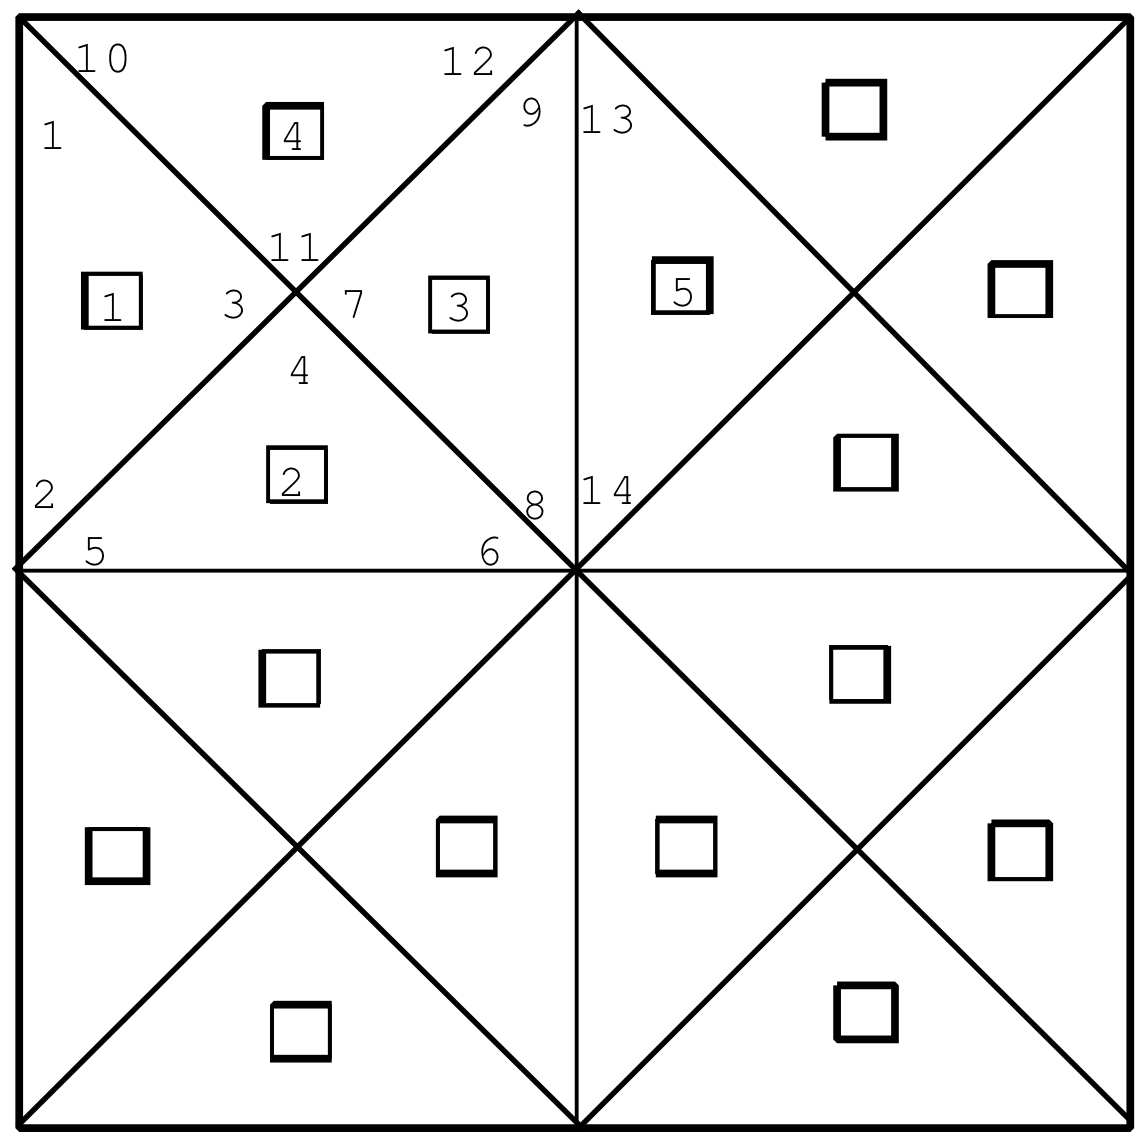
\includegraphics[height=5cm]{images/discretisation.png}
\caption{Section de la poutre discrétisée en triangles}
\label{fig:discretisation}
\end{figure}


\newpage
\section{Modélisation}
Soit $L$ la longueur d'un côté de la poutre. On défini $l=\frac{L}{N}$, la longueur d'un côté d'un triangle et $h=\frac{l}{2}$, la longueur de la hauteur. On considère quatre cas : 
\begin{itemize}
\item cas triangle 1, orienté comme le 1 sur la figure \ref{fig:discretisation};
\item cas triangle 2, orienté comme le 2 sur la figure \ref{fig:discretisation};
\item cas triangle 3, orienté comme le 3 sur la figure \ref{fig:discretisation};
\item cas triangle 4, orienté comme le 4 sur la figure \ref{fig:discretisation};
\end{itemize} 
et dans chacun des cas, on écrit les conditions de divergence nulle comme une différence finie. Pour les conditions de continuité, on distingue 

\begin{align*}
\frac{\sigma_{xx}^3 - \frac{\sigma_{xx}^1+\sigma_{xx}^2}{2}}{h} + \frac{\sigma_{xy}^1-\sigma_{xy}^2}{l}&=0 & \text{pour triangle type 1}\\
\frac{\sigma_{xy}^3 - \frac{\sigma_{xy}^1+\sigma_{xy}^2}{2}}{h} + \frac{\sigma_{yy}^1-\sigma_{yy}^2}{l}&=0& \text{pour triangle type 1}\\
\frac{\sigma_{xx}^3-\sigma_{xx}^2}{l} + \frac{\sigma_{xy}^1 - \frac{\sigma_{xy}^3+\sigma_{xy}^2}{2}}{h} &=0& \text{pour triangle type 2}\\
\frac{\sigma_{xy}^3-\sigma_{xy}^2}{l} + \frac{\sigma_{yy}^1 - \frac{\sigma_{yy}^3+\sigma_{yy}^2}{2}}{h} &=0 & \text{pour triangle type 2}\\
\frac{\frac{\sigma_{xx}^3+\sigma_{xx}^2}{2} - \sigma_{xx}^1 }{h} + \frac{\sigma_{xy}^3-\sigma_{xy}^2}{l}&=0& \text{pour triangle type 3}\\
\frac{\frac{\sigma_{xy}^3+\sigma_{xy}^2}{2} - \sigma_{xy}^1 }{h} + \frac{\sigma_{yy}^3-\sigma_{yy}^2}{l}&=0& \text{pour triangle type 3}\\
\frac{\sigma_{xx}^3-\sigma_{xx}^1}{l} + \frac{\frac{\sigma_{xy}^1+\sigma_{xy}^3}{2} - \sigma_{xy}^2 }{h} &=0 & \text{pour triangle type 4}\\
\frac{\sigma_{xy}^3-\sigma_{xy}^1}{l} + \frac{\frac{\sigma_{yy}^1+\sigma_{yy}^3}{2} - \sigma_{yy}^2 }{h} &=0 & \text{pour triangle type 4}\\
\end{align*}



%\begin{align}
%\max \sum_{j \in \text{top nodes, $x_j < x_{j+1}$}} \frac{|\sigma_{yy}^j - \sigma_{yy}^{j+1}|}{2 d } & \\
%\frac{\sigma_{xx}^n - \sigma_{xx}^m}{x_n - x_m}  + \frac{\sigma_{xx}^p - \sigma_{xx}^m}{x_p - x_m} + \frac{\sigma_{xy}^n - \sigma_{xy}^m}{y_n - y_m} + \frac{\sigma_{xy}^p - \sigma_{xy}^m}{y_p - y_m} &= 0  & \forall \triangle j, \forall \text{noeud $1$, $2$ et $3$} \in \triangle_j \\
%\frac{\sigma_{xy}^n - \sigma_{xy}^m}{x_n - x_m}  + \frac{\sigma_{xy}^p - \sigma_{xy}^m}{x_p - x_m} + \frac{\sigma_{yy}^n - \sigma_{yy}^m}{y_n - y_m} + \frac{\sigma_{yy}^p - \sigma_{yy}^m}{y_p - y_m} &= 0  & \forall \triangle j, \forall \text{noeud $1$, $2$ et $3$} \in \triangle_j \\
%\sigma_{xx}^i &= \sigma_{xx}^j & \text{si le noeud (i) et (j) sont confondus}\\
%\sigma_{xy}^i &= \sigma_{xy}^j & \text{si le noeud (i) et (j) sont confondus}\\
%\sigma_{yy}^i &= \sigma_{yy}^j & \text{si le noeud (i) et (j) sont confondus}\\
%\sigma_{xx}^i &= 0 & \text{si le noeud (i) est sur la frontière} \\
%\sigma_{xy}^i &= 0 & \text{si le noeud (i) est sur la frontière}\\
%(\sigma_{xx}^i - \sigma_{yy}^i)^2 + (2 \sigma_{xy}^i)^2 & \leq 4 k^2 & \forall \text{noeud $i$}
%\end{align}


